% Document class and parameters %
\documentclass[10pt,a4paper]{article}

% Document packages %
\usepackage{graphicx}
\usepackage{biblatex}
\usepackage{parskip}
\usepackage{listings}
\usepackage{caption}
\usepackage{subcaption}
\usepackage{amsmath}
\usepackage{amssymb}
\usepackage[most]{tcolorbox}
\usepackage{wrapfig}


% Parameters %
\lstset{basicstyle=\ttfamily, breaklines = true, tabsize=2}
\graphicspath{{./Images/}}
\setlength{\parskip}{1em}

% Document Body %
\begin{document}
\begin{titlepage}
	\centering
	{\scshape\LARGE Imperial College London \par}
	\vspace{1cm}
	{\scshape\Large Mathematics: Year 2\par}
	\vspace{1.5cm}
	{\huge\bfseries Complex Variables\par}
	\vspace{2cm}
	{\Large\ Xin Wang }
	\vfill
	{\large \today\par}
\end{titlepage}

\begin{abstract}
Complex variables, just like Real and Natural numbers, were invented as a way to make calculations
simpler. While numerical analysis is used in modern day, complex variables still plays an important
role in Electrical Engineering as means to simplify calculations as seen with Fourier and Laplace. \par 

Many of the theory builds on existing Complex Numbers covered previously - a revision topic focuses
on the abstract meaning of complex numbers.
\end{abstract}

\tableofcontents
\pagebreak

% Sections Body %
\section{Revision}

%%%%%%%%%%%%%%%%%%%%%%%%%%%%%%%%%%%%%%%%%%%%%%%%%%%%%%%%%%%%%%%%%%%%%%%%%%%%%%%%%%%%%%%%%%%%%%%%%%%%%%%%%%
\subsection{Complex Numbers}

Complex numbers $\mathbb{C}$ are defined as points in a plane meaning that it is 2-D number system
compared to real numbers $\mathbb{R}$ which is a 1-D number system i.e. a line. The 2-D system
allows it to be easily described through the use of matrices.

\begin{tcolorbox}[breakable,colback=white]
\textbf{Complex plane} ($\mathbb{C}$): A geometric representation of the complex
numbers established by the \textbf{real axis} and the \textbf{imaginary axis}.
\\
\\
\textbf{Complex analysis}: The branch of mathematical analysis that investigates functions of
complex numbers.
\\
\\
\textbf{Complex numbers}: A number that can be expressed in the form $a+bi$ where $a$ and $b$ are
real numbers and $i$ represents the imaginary unit satisfying $i^2=-1$.
\end{tcolorbox}

The matrix form can be compressed into the form $a+ib$ usually seen. It should be noted
that \textit{real} and \textit{imaginary} are purely just terminology used only due to historical
reasons. Imaginary numbers are just as real as Real numbers as it \textbf{is only a system to
address certain equations that have no solutions}.

%%%%%%%%%%%%%%%%%%%%%%%%%%%%%%%%%%%%%%%%%%%%%%%%%%%%%%%%%%%%%%%%%%%%%%%%%%%%%%%%%%%%%%%%%%%%%%%%%%%%%%%%%%
\subsection{Complex Functions}

The basic concept of a function involves two sets $X$ and $Y$ and each element ($x$ - \textbf{independent
variable}) in $X$ maps to an element ($y$ - \textbf{dependent variable})
in $Y$: $$y=f(x)$$ where ($x\in X$) \par 

A \textbf{complex function} is a function such that the independent variable $z$ is a complex variable $z=x+iy$ where $x$ and
$y$ are real numbers. If the independent variable is a complex variable, the dependent variable $w$ is
usually also a complex number: 
$$w=f(z)=u+jv$$
All the complex function details cannot be plotted like a normal Cartesian $y=f(x)$ plot. The values
are instead plotted \textbf{on two separate planes}: $z$-plane (independent variable) and $w$-plane (dependent variable)
\begin{figure} [h!]
    \centering
    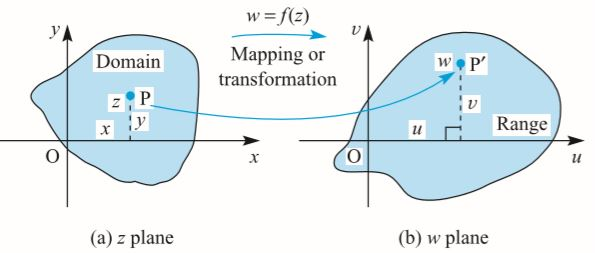
\includegraphics[scale=0.5]{Z-plane}
\end{figure}

\pagebreak

%%%%%%%%%%%%%%%%%%%%%%%%%%%%%%%%%%%%%%%%%%%%%%%%%%%%%%%%%%%%%%%%%%%%%%%%%%%%%%%%%%%%%%%%%%%%%%%%%%%%%%%%%%
\section{Analyticity and Cauchy-Riemann equations}

As encountered previously, an analytic function is a function that can be approximated by a Taylor
power series. The relation between analyticity, Taylor series and complex variables are rooted in
understanding if a function can be evaluated. It is a common problem in mathematics when dealing
with functions. 

The fundamental basic tools mathematicians have for function evaluation are the four arithmetic
operations $+,-,\times,\div$ In summary, the study of polynomials is basically the study of
\textit{ "what can we do with basic arithmetic?"} So when it is proven that a function can be
approximated by a Taylor series i.e. being analytic, it means that the function can be evaluated to
a desired precision via basic arithmetic.

So in complex analysis, analyticity and its associated properties are critical.

Suppose that a function of a complex number $z$
\begin{align*}
    f(z) = u(z) + \text{i} v(z)
\end{align*}

Then the complex derivative of $f$ at a point $z_0$ is defined by:

$$f^{\prime}(z_0)=\lim_{h\rightarrow 0}\left[\frac{f(z_0 + h)-f(z_0)}{h}\right]$$
provided this limit exists. 

\textbf{If this limit does exists}, then it may be computed by taking the limit as $h \rightarrow 0$ along
the real axis or the imaginary axis. Either case \textbf{it should give the same result}. Approaching along
the real axis $x$:  

$$\lim_{h\rightarrow 0}\left[\frac{f(z_0 + h)-f(z_0)}{h}\right]=\frac{\partial f}{\partial x}(z_0)$$

On the other hand, approaching along the imaginary axis $y$:
$$\lim_{h\rightarrow 0}\left[\frac{f(z_0 +
\text{i}h)-f(z_0)}{\text{i}h}\right]=\frac{1}{\text{i}}\frac{\partial f}{\partial y}(z_0)$$

The equality of the derivative of $f$ taken along the two axis is:
$$\frac{\partial f}{\partial y}(z_0)=\text{i}\frac{\partial f}{\partial x}(z_0)$$
which are the Cauchy–Riemann equations at the point $z_0$.

The difference compared to real variables is that the point $z_0$ is on a plane and can be approached along an
infinite number of curves in the $z$ plane. This means that the existence of a unique limit is not easily
verified but it is still an important requirement to prove a function can be evaluated.

\pagebreak
%%%%%%%%%%%%%%%%%%%%%%%%%%%%%%%%%%%%%%%%%%%%%%%%%%%%%%%%%%%%%%%%%%%%%%%%%%%%%%%%%%%%%%%%%%%%%%%%%%%%%%%%%%
\subsection{Cauchy-Riemann equations}

As noted above, any analytic function (real or complex) is \textbf{infinitely differentiable} i.e.
smooth or $C^{\infty}$.

\begin{tcolorbox}[breakable,colback=white]
    \textbf{Analytic \textit{in $R$}}: The function $f(z)$ has a derivative $f^{\prime}(z)$ that exists at all points of
    a region $R$ of the $z$ plane. Can also be defined as: \textbf{Regular} or \textbf{Holomorphic}.
\end{tcolorbox}

Though the term \textbf{analytic function} is often used interchangeably with \textbf{holomorphic
function}, the word "analytic" is defined in a broader sense to denote any function (real, complex,
or of more general type) that can be written as a convergent power series in a neighbourhood of each
point in its domain i.e. all points can be approximated. The fact that all holomorphic functions are
complex analytic functions, and vice versa, is a major theorem in complex analysis.

As mentioned earlier that the existence of an \textbf{unique limit} is required and, in order for
there to be an \textbf{unique} limit, the limit needs to be independent of the direction in which the limit
is taken. \par

The easiest way to check whether it is independent of the direction of the limit is to establish the
\textbf{Cauchy-Riemann equations}. \par 

\begin{tcolorbox}[breakable,colback=white]
If $z=x+iy$ and $f(z)=u(x,y)+iv(x,y)$, and $f(z)$ is analytic in some region $R$ of the $z$-plane
then: 
\begin{equation}
    \frac{\partial u}{\partial x}=\frac{\partial v}{\partial y} \equiv u_x = v_y
\end{equation}
\begin{equation}
    \frac{\partial u}{\partial y}=-\frac{\partial v}{\partial x} \equiv u_y = -v_x
\end{equation}
where (1) and (2) are the \textbf{Cauchy-Riemann equations} and holds throughout $R$
\end{tcolorbox}

Some functions are analytic everywhere in the complex plane except at certain points
i.e. \textbf{singularities} - where the limit not does exist.

%%%%%%%%%%%%%%%%%%%%%%%%%%%%%%%%%%%%%%%%%%%%%%%%%%%%%%%%%%%%%%%%%%%%%%%%%%%%%%%%%%%%%%%%%%%%%%%%%%%%%%%%%%
\subsubsection{Derivation of Cauchy-Riemann equations}

A general test is performed on functions to determine if the function is independent of the
direction of the limit: \par 

Given: 
$$f(z)=u(x,y)+iv(x,y)$$
Take the limit in the horizontal direction ($\partial z = \partial x$):
$$\frac{df(z)}{dz}=\frac{\partial u}{\partial x}+i\frac{\partial v}{\partial x} \equiv u_x + iv_x$$

Take the limit in the vertical direction ($\partial z = i\partial y$):
\begin{equation*}  
    \begin{aligned}
        \frac{df(z)}{dz} &= \frac{\partial u}{\partial (iy)}+i\frac{\partial v}{\partial (iy)} \\
        &= -i\frac{\partial u}{\partial y} + \frac{\partial v}{\partial y} \equiv -iu_y + iv_y
    \end{aligned}
\end{equation*}

\textbf{Example 1}: Given $f(z)=z^{-1}$, determine the analyticity of the equation. \par 
Expressing $z$ as:
$$z^{-1}=\frac{(x-iy)}{x^2 + y^2}$$
Two equations obtained are: 
$$u(x,y)=\frac{x}{x^2+y^2}$$
$$v(x,y)=-\frac{y}{x^2+y^2}$$
It is easy to see that Cauchy-Riemann equations hold everywhere except at origin $z=0$ where the
limit is indeterminate - the point (Singularity) at where it fails to be differentiable. \par 

\textbf{Example 2}: Given $f(z)=z^2$, determine the analyticity of the equation. \par 
Expressing $z^2$ as:
$$z^{2}=x^2 - y^2 + 2ixy$$
Two equations obtained are: 
$$u(x,y)={x^2-y^2}$$
$$v(x,y)=2xy$$
The four partial derivatives are:
$$u_x=2x$$
$$u_y=-2y$$
$$v_x=2y$$
$$v_y=2x$$
This indicates that the equation is differentiable at all points in the $z$-plane - analytic
everywhere. 

%%%%%%%%%%%%%%%%%%%%%%%%%%%%%%%%%%%%%%%%%%%%%%%%%%%%%%%%%%%%%%%%%%%%%%%%%%%%%%%%%%%%%%%%%%%%%%%%%%%%%%%%%%
\subsection{Properties of analytic functions}

If functions satisfies the Cauchy-Riemann equations, these functions are also:
\begin{enumerate}
    \item Harmonic functions
    \item Conjugate functions
\end{enumerate}

%%%%%%%%%%%%%%%%%%%%%%%%%%%%%%%%%%%%%%%%%%%%%%%%%%%%%%%%%%%%%%%%%%%%%%%%%%%%%%%%%%%%%%%%%%%%%%%%%%%%%%%%%%
\subsubsection{Conjugate functions}

Conjugate functions satisfy the \textbf{orthogonality property}. The curves in the $x,y$-plane
defined by $u(x,y)=\text{constant}$ and $v(x,y)=\text{constant}$ are orthogonal: 
\begin{equation*}
    \left[\frac{dy}{dx}\right]_u = -\frac{\frac{\partial u}{\partial y}}{\frac{\partial u}{\partial x}} \text{   and   } 
    \left[\frac{dy}{dx}\right]_v = -\frac{\frac{\partial v}{\partial y}}{\frac{\partial v}{\partial x}}
\end{equation*}
\begin{equation*}
    \left[\frac{dy}{dx}\right]_u \times \left[\frac{dy}{dx}\right]_v = -1
\end{equation*}

Conjugate functions form the basis of forming contour maps.

%%%%%%%%%%%%%%%%%%%%%%%%%%%%%%%%%%%%%%%%%%%%%%%%%%%%%%%%%%%%%%%%%%%%%%%%%%%%%%%%%%%%%%%%%%%%%%%%%%%%%%%%%%
\subsubsection{Harmonic functions}

\begin{tcolorbox}[breakable,colback=white]
    Harmonic functions satisfies \textbf{Laplace's equation} in two dimension:
    \begin{equation*}
        \frac{\partial^2u}{\partial x^2} + \frac{\partial^2u}{\partial y^2}=0
    \end{equation*}

    By satisfying Laplace's equation, it shows that function $v$ exists and can be found.
\end{tcolorbox}

As functions satisfying the Cauchy-Riemann equations are analytic hence the functions are also
harmonic functions. \par 
The name harmonic function originates from a point on a taut string which is undergoing harmonic
motion. The solution to the differential equation for this type of motion can be written in terms of
sines and cosines, functions which are thus referred to as harmonics. Harmonic functions have applications in areas such as stress analysis and fluid flow.

\textbf{Example 1}: Given the function $u=x^2 - y^2$, show 
\begin{itemize}
    \item Function is harmonic:
    
    From the equation above: $u_x = 2x$, $u_y=-2y$, $u_{xx}=2$ and $u_{yy}=-2$:
    $$u_{xx}+u_{yy}=0$$
    hence satisfying the Laplace equation, indicating it is a Harmonic function.

    \item Find $v(x,y)$:
    
    As $v$ exists, it is defined by $v_y=u_x=2x$ and $v_x=-u_y=2y$. Using integration, $v$ is found:
    \begin{equation*} 
    v=2xy+A(x) \textrm{   and   } v=2xy+B(y) 
    \end{equation*}
    \begin{equation*} 
    v=2xy+c
    \end{equation*}
    where $c$ is a constant to be defined by conditions set out initially

    \item Construct the corresponding complex function $f(z)$:
    
    \begin{equation*} 
        \begin{aligned}
            f(z)&=x^2-y^2 \\
            &= 2ixy + ic \\
            &= z^2 + ic 
        \end{aligned}
        \end{equation*}
\end{itemize}

\textbf{Example 2}: Given that $u=x^3-3xy^2$, find:
\begin{itemize}
    \item Find conjugate function $v(x,y)$:
    \begin{enumerate}
        \item Check that $u=x^3-3xy^2$ satisfies Laplace's equation to ensure $v$ exists.
            \begin{align*}
                u_x &= 2x^2-3y^2\; \text{ and }\; u_{xx}=6x \\
                u_y &= -6xy \;\text{ and }\; u_{yy}=-6x 
            \end{align*}
            Equate as $u_{xx}+u_{yy}$:
            \begin{align*}
                u_{xx}+u_{yy} = 6x + (-6x) = 0
            \end{align*}
            Satisfies Laplace's equation hence $v$ exists.

        \item Find $v$ from Cauchy-Riemann equations:
        \begin{align*}
            v_y &= 3x^2 - 3y^2 \\
            v_x &= 6xy 
        \end{align*}
        Integrate:
        \begin{align*}
            v &= 3x^2y - y^3 + A(x) \\
            v &= 3x^2y + B(y)
        \end{align*}
        Choose $A(x) = c$ and $B(y)=-y^3+c$:
        $$
            v = 3x^2y - y^3 + c
        $$
    \end{enumerate}

    \item Corresponding complex function $f(z)$:
    \begin{align*}
        f(z) &= x^3 - 3xy^2 + i(2x^2y - y^3 + c) \\
        &= z^3 + ic 
    \end{align*}
\end{itemize}

\pagebreak

%%%%%%%%%%%%%%%%%%%%%%%%%%%%%%%%%%%%%%%%%%%%%%%%%%%%%%%%%%%%%%%%%%%%%%%%%%%%%%%%%%%%%%%%%%%%%%%%%%%%%%%%%%
\section{Mappings}

As with functions, it is very useful to be able to graphically express a function. However, complex
functions cannot be plotted on the complex plane since one would need four dimensions:
\begin{itemize}
    \item Two inputs to plot: Real and Imaginary 
    \item Two outputs to plot: Real and Imaginary
\end{itemize}

But, there are several possible ways to get around the problem:
\begin{itemize}
    \item Separately plot the \textbf{real} and \textbf{imaginary} components.
    \item Express complex variables as an \textbf{argument} and \textbf{absolute} value. 
\end{itemize}

However, more commonly, a more primitive method called \textbf{mappings} or \textbf{transformations}
is used. The $z$-plane and its points are inputted into a specified complex function and
resulting values are plotted in the $w$-plane. 

Commonly described as \textit{mapping of $z$ to $w$} or \textit{$w$ is the image of $z$}.
\begin{align*}
    w = f(z)
\end{align*}

For example, under the mapping $z \mapsto iz$, the image of the \textbf{imaginary} $z$-axis is the
\textbf{real} $w$-axis
\begin{figure} [h!]
    \centering
    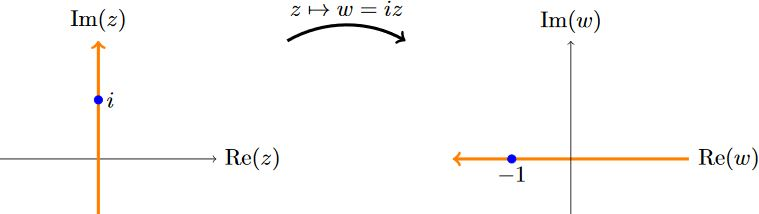
\includegraphics[scale=0.7]{Map meaning.JPG}
\end{figure}

This change of shape during course of the transition gives mathematicians details on how the
fundamental function behaves. It is fundamentally this feature of complex mappings that allows
complex functions to have so much potential applications in various engineering fields.

Common notations used:
\begin{itemize}
    \item Domain $z=x+iy$: The initial $z$-plane.
    \item Range $w=u+iv$: The mapped $w$-plane.
    \item $w=f(z)$: The equation indicating $z$-plane is mapped to $w$-plane.
\end{itemize}

\pagebreak

%%%%%%%%%%%%%%%%%%%%%%%%%%%%%%%%%%%%%%%%%%%%%%%%%%%%%%%%%%%%%%%%%%%%%%%%%%%%%%%%%%%%%%%%%%%%%%%%%%%%%%%%%%
\subsection{Conformal Mapping}

As mentioned earlier, studying this transformation process allows engineers to find potential
applications to engineering problems. One of the aspects of the mapping process is that \textbf{the
mapping may not be unique} i.e. given the transformation $w=z^2$, the two values $\pm z_0$ maps to
only one value $w_0$ thus showing that the function is not a one-to-one.

This aspect has potential ramifications since one-to-one functions are a common condition in
engineering systems so there must be a condition to ensure the mapping is one-to-one. Recall the
concept of \textbf{analytic functions} - an important property of an analytic function is its
uniqueness i.e. a value in the $z$-domain maps to a value in the $w$-plane.

Using the concepts of analytic functions, an important property within mappings is developed called \textbf{conformality}.

\begin{tcolorbox}[breakable,colback=white]
\textbf{Conformal mapping}: A mapping $w=f(z)$ that preserves angles in both magnitude and sense.
\begin{itemize}
    \item \textbf{Magnitude}: Angle between two intersecting curves in $z$-plane is the same as
    angle between corresponding intersecting curves in the $w$-plane.
    \item \textbf{Sense}: Given $\theta$, the angle between curves take in the anti-clockwise sense
    in $z$-plane then $\theta$ is also the angle between image of curves in the $w$-plane also taken in
    anti-clockwise sense.
\end{itemize}
\end{tcolorbox}
\begin{figure} [h!]
    \centering
    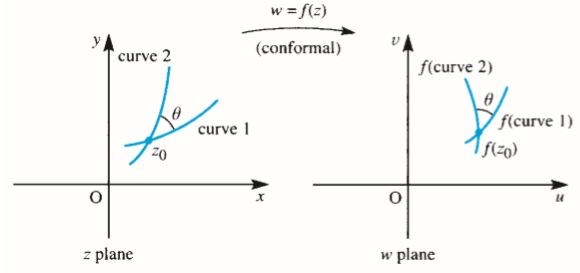
\includegraphics[scale=0.9]{sense and angle.JPG}
    \caption{Conformal mapping showing magnitude and sense}
\end{figure}

Conformal mappings are invaluable for solving problems in engineering and physics that can be
expressed in terms of functions of a complex variable yet exhibit inconvenient geometries. By
choosing an appropriate mapping, the analyst can transform the inconvenient geometry into a much
more convenient one while maintaining the critical details of the problem.

\pagebreak

A mapping has a \textbf{fixed point} i.e. a point that remains the same throughout the
transformation process: \par 
$$
    w=f(z)=z
$$ 
Note that though a mapping defined by an analytic function, the resulting transformation $w=f(z)$ is
\textbf{not conformal everywhere}. There are points where the analytic characteristic fails called
\textbf{singularities}:
\begin{align*}
    f'(z)=0
\end{align*} 

\textbf{Example 1}: Given $w=z^2$ and $f^{\prime}=2z$, describe the mapping. \par 
The mapping is conformal everywhere except at $z=0$ because $f'(0)=2(0)=0$, conformality fails at the
origin which means the orthogonality property also fails. \par
\begin{figure} [h!]
    \centering
    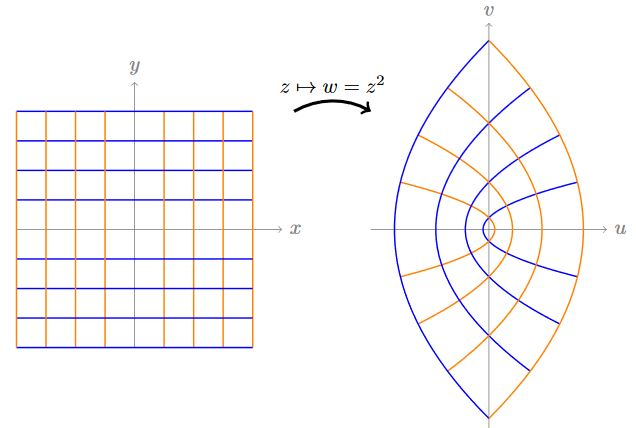
\includegraphics[scale=0.7]{conformal.JPG}
    \caption{Transformation $w=z^2$}
\end{figure}
This transformation maps the horizontal and vertical grid lines to mutually orthogonal parabolas.
$f(z)$ is conformal so the orthogonality of the parabolas is no accident. This shows that the
conformal map preserves the right angles between the grid lines.

\pagebreak

%%%%%%%%%%%%%%%%%%%%%%%%%%%%%%%%%%%%%%%%%%%%%%%%%%%%%%%%%%%%%%%%%%%%%%%%%%%%%%%%%%%%%%%%%%%%%%%%%%%%%%%%%%
\subsection{Linear transformation}

The general complex linear function
\begin{align*}
    w = \alpha z + \beta
\end{align*}
where:
\begin{itemize}
    \item $w$ and $z$ are complex-valued variables
    \item $\alpha$ and $\beta$ are complex constants
\end{itemize}  

It is of interest to study the mappings of the $z$ plane onto the $w$ plane for different choices of
the constants $\alpha$ and $\beta$. In so doing, some general properties of mappings are revealed.

%%%%%%%%%%%%%%%%%%%%%%%%%%%%%%%%%%%%%%%%%%%%%%%%%%%%%%%%%%%%%%%%%%%%%%%%%%%%%%%%%%%%%%%%%%%%%%%%%%%%%%%%%%
\subsubsection{$\alpha = 0$}

Letting $\alpha = 0$
\begin{align*}
    w = \beta
\end{align*}

This mapping implies that $w = \beta$ no matter what the value of $z$. This is obviously a
\textbf{degenerate mapping} i.e. the entire $z$ plane is being mapped onto the one point $w = \beta$
in the $w$ plane.
\begin{figure} [h!]
    \centering
    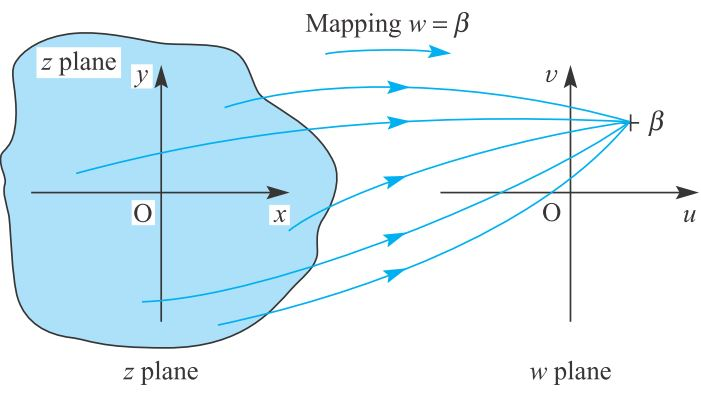
\includegraphics[scale=0.3]{Degenerate mapping.JPG}
    \caption{Degenerate mapping}
\end{figure}

The point $\beta$ is a fixed point in this mapping. Note that this mapping has no inverse since it is
not analytic.

\pagebreak

%%%%%%%%%%%%%%%%%%%%%%%%%%%%%%%%%%%%%%%%%%%%%%%%%%%%%%%%%%%%%%%%%%%%%%%%%%%%%%%%%%%%%%%%%%%%%%%%%%%%%%%%%%
\subsubsection{$\beta=0$ and $\alpha \neq 0$}

Letting $\beta=0$ and $\alpha \neq 0$
\begin{align*}
    w = \alpha z
\end{align*}

Under this mapping, the origin is the only fixed point, there being no other fixed points that are
finite. Also, in this case there exists an inverse mapping
\begin{align*}
    z = \frac{1}{\alpha}w
\end{align*}

This mapping has the following effects:
\begin{itemize}
    \item Maps the origin in the $z$ plane to the origin in the $w$ plane i.e. fixed point
    \item \textbf{Magnification}: Expands mapping  by $|\alpha|$ 
    \item \textbf{Rotation}: Rotates anticlockwise by $arg(\alpha)$
\end{itemize}
\begin{figure} [h!]
    \centering
    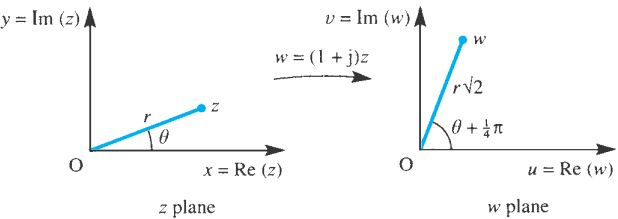
\includegraphics[scale=0.7]{betaal.JPG}
    \caption{Magnification and rotation}
\end{figure}

Certain properties in linear mappings are preserved, the most important being that straight lines in
the $z$ plane will be transformed to straight lines in the $w$ plane. Likewise, circles are mapped onto circles.

Note the above example does not include any translation since $\beta = 0$
\begin{figure} [h!]
    \centering
    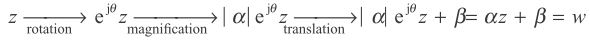
\includegraphics[scale=0.8]{TR.JPG}
    \caption{Summary of the effects of different variables}
\end{figure}

\pagebreak

%%%%%%%%%%%%%%%%%%%%%%%%%%%%%%%%%%%%%%%%%%%%%%%%%%%%%%%%%%%%%%%%%%%%%%%%%%%%%%%%%%%%%%%%%%%%%%%%%%%%%%%%%%
\subsection{Reciprocal transformation: $w=\frac{1}{z}$}

As mentioned previously, studying a transformation gives clues on how transformations can be used.
This transformation is also a one-to-one correspondence between the nonzero points of the $z$ and $w$
planes.

An interesting property of this mapping $w=\frac{1}{z}$ is considering the image of circles and
straight lines in the $z$ plane under such a mapping.

Every circle or line in the $z$-plane can be described by the general equation:
\begin{align*}
    Ax+By+C(x^2+y^2) =D
\end{align*}
where if $C = 0$ then it is a straight line and if $C \neq 0$ then it is a circle.

This general equation in the $z$-plane can be converted into another equation in the $w$-plane:
\begin{align*}
    Au - Bv + C = D(u^2 + v^2)
\end{align*}

This shows that a line or circle in $x,y$ is transformed to a line or circle in $u,v$, meaning that inversion maps lines and circles to lines and circles.

Several properties of this transformation:
\begin{enumerate}
    \item Any line not through the origin is mapped to a circle through the origin.
    \item Any line through the origin is mapped to a line through the origin.
    \item Any circle not through the origin is mapped to a circle not through the origin.
    \item Any circle through the origin is mapped to a line not through the origin.
\end{enumerate}

The value of $\alpha$ and $\Delta$ affects the mapping of lines and circles:
\begin{itemize}
    \item $C = 0$: Transformation results in lines
    \item $C \neq 0$: Transformation results in circles
\end{itemize}


\pagebreak

%%%%%%%%%%%%%%%%%%%%%%%%%%%%%%%%%%%%%%%%%%%%%%%%%%%%%%%%%%%%%%%%%%%%%%%%%%%%%%%%%%%%%%%%%%%%%%%%%%%%%%%%%%
\subsection{Fractional linear transformation}

A fractional linear transformation or \textbf{Mobius} transformation is a function of the form:
\begin{align*}
    w=\frac{az+b}{cz+d}
\end{align*}
where $a$, $b$, $c$, $d$ are complex constants and $ad-bc \neq 0$

\textbf{Simple point}: If $ad-bc= 0$ then $w$ is a constant function.

A Mobius transformation maps lines/circles to lines/circle with contraction, rotation and
translation. \par 
This transformation includes cases such as:
\begin{enumerate}
    \item $w=\frac{1}{z}$ when $a=d=0$ and $\frac{b}{c}=1$
    \item $w\frac{1}{z-1}$ when $a=0$, $b=1$, $c=1$ and $d=-1$
\end{enumerate}

The above equation can be written as:
$$w=c^{-1}\left\{a+\frac{bc-ad}{cz+d}\right\}$$
The special cases are defined as:
\begin{enumerate}
    \item $w=z+b$ where $a=d=1$ and $c=0$: \textbf{Translation}
    \item $w=az$ where $b=c=0$ and $d=1$: \textbf{Contraction + Rotation}
    \item $w=\frac{1}{z}$ where $a=d=0$ and $b=c$: \textbf{Lines/Circles to Lines/Circles}
\end{enumerate}

\pagebreak

%%%%%%%%%%%%%%%%%%%%%%%%%%%%%%%%%%%%%%%%%%%%%%%%%%%%%%%%%%%%%%%%%%%%%%%%%%%%%%%%%%%%%%%%%%%%%%%%%%%%%%%%%%
\subsection{Example Questions}

\textbf{Example 1}: Given the complex mapping from $z=x+iy$ to $w=u+iv$:
\begin{align*}
    w = \frac{1}{z + i}
\end{align*}
\begin{itemize}
    \item Show that circles $x^2+(y+1)^2=a^2$ in the $z$-plane map to circles in the $w$-plane, and
    give the equation of the circles in terms of $u,v$.
    \begin{align*}
        u + iv &= \frac{1}{x + iy + i} \\
        &= \frac{x - i(y+1)}{x^2 + (y+1)^2} \\
    \end{align*}
    Splitting between real and imaginary: 
    \begin{align*}
        u = \frac{x}{x^2 + (y+1)^2} \; \text{ and } \; v = \frac{-y+1}{x^2 + (y+1)^2}
    \end{align*}
    Circle formula:
    \begin{align*}
        u^2+v^2 &= \left[\frac{x}{x^2 + (y+1)^2}\right]^2 + \left[\frac{-y+1}{x^2 + (y+1)^2}\right]^2 \\
        &= \frac{1}{x^2 + (y+1)^2} \\
        &= \frac{1}{a^2}
    \end{align*}

    \item Show that the axes in the $z$-plane map to an axis and a circle in the $w$-plane. Obtain the axis and circle.
    
    y-axis: $x=0$
    \begin{align*}
        w &= \frac{1}{x+iy+i} \\
        &= \frac{1}{0 + iy + i} \\
        &= \frac{1}{i(y+1)} \\
        v &= \frac{1}{y+1}
    \end{align*}

    x-axis: $y=0$
    \begin{align*}
        w &= \frac{1}{x+iy+i} \\
        &= \frac{1}{x + 0 + i} \\
        &= \frac{1}{x+i} \\
        &= \frac{x-i}{x^2+1}
    \end{align*}

    Use the circle formula:
    \begin{align*}
        u^2 + v^2 &= \left[\frac{x}{x^2 + 1}\right]^2 + \left[\frac{-1}{x^2 + 1}\right]^2 \\
        &= \frac{1}{x^2 + 1} \\
        &= -v 
    \end{align*}

    Simplify:
    \begin{align*}
        u^2 + v^2 + v &= 0 \\
        u^2 + \left(v+\frac{1}{2}\right)^2 &= \frac{1}{4}
    \end{align*}

    \item Obtain the images in $w$ of the lines $y=x-1$ and $y=-1$.
    \begin{itemize}
        \item $y=x-1$ and $x=y+1$:
        \begin{align*}
            z &= x+ iy            
        \end{align*}
        Split:
        \begin{align*}
            u = \frac{x}{x^2 + (y+1)^2} \; &\text{ and } \; v = \frac{-y+1}{x^2 + (y+1)^2} \\ 
            u = \frac{1}{2(y+1)} \; &\text{ and } \; v = \frac{-1}{2(y+1)}
        \end{align*}

        \item $y=-1$:
        \begin{align*}
            w &= \frac{1}{x+i(y+1)} \\
            &= \frac{1}{x}
        \end{align*}
    \end{itemize}

\end{itemize}






\pagebreak

%%%%%%%%%%%%%%%%%%%%%%%%%%%%%%%%%%%%%%%%%%%%%%%%%%%%%%%%%%%%%%%%%%%%%%%%%%%%%%%%%%%%%%%%%%%%%%%%%%%%%%%%%%
\section{Singularities, Zeroes and Residues}

In order to see how singularities contribute to complex integrals, methods to find their nature and
classification is required.

%%%%%%%%%%%%%%%%%%%%%%%%%%%%%%%%%%%%%%%%%%%%%%%%%%%%%%%%%%%%%%%%%%%%%%%%%%%%%%%%%%%%%%%%%%%%%%%%%%%%%%%%%%
\subsection{Singularities and Zeroes}

\begin{tcolorbox}[breakable,colback=white]
\textbf{Singularity} (of a complex function $f(z)$): A point of the $z$-plane where $f(z)$ ceases to
be analytic - a point where the mathematical object ceases to be
well-behaved, such as the lack of differentiability or analyticity e.g.
$f(z)=\frac{1}{x}$ where a singularity is $x=0$. 
\\
\\
\textbf{Zero} (of a complex function $f(z)$): A point in the $z$-plane at which $f(z) = 0$.
\\
\\
\textbf{Poles} (of a complex function $f(z)$): A zero of $\frac{1}{f}$. 
\end{tcolorbox}

Singularities of complex functions has many classifications and the simplest class is: \textbf{Simple Poles}
(Order of 1). \par

A function has a simple pole at a point $a$ if it can be written in the form: 
$$
f(z)=\frac{g(z)}{z-a}
$$
where $g(z)$ is an analytic function

%%%%%%%%%%%%%%%%%%%%%%%%%%%%%%%%%%%%%%%%%%%%%%%%%%%%%%%%%%%%%%%%%%%%%%%%%%%%%%%%%%%%%%%%%%%%%%%%%%%%%%%%%%
\subsection{Residue} 

\begin{tcolorbox}[breakable,colback=white]
\textbf{Meromorphic}: A function that is analytic on except for a set of poles of finite order.
\\
\\
\textbf{The residue $Res(f,c)$} (of a function $f(z)$ at $c$): The coefficient of $(z-c)^{-1}$
resulting from the Laurent series expansion off at point $c$.
\end{tcolorbox}

Residue of a pole is important in integration, once known, allow the determination of general
contour integrals via the residue theorem. Contour integration is a method of evaluating certain
integrals along paths in the complex plane and it is closely related to residue of a complex function. 

There are more efficient ways of calculating the residue than finding the Laurent series expansion.
\begin{enumerate}
    \item Residue of $f(z)$ at a simple pole at $z=a$:
    $$
        \text{Residue of }f(z) = \lim_{z\rightarrow a}{(z-a)f(z)}
    $$
    \item Residue of $f(z)$ at a pole of multiplicity at $z=a$: (Formula provided)
    $$
        \text{Residue of }f(z) = \lim_{z\rightarrow a}\left[\frac{1}{(m-1)!}\times \frac{d^{m-1}}{dz^{m-1}} \times [z-a]^m \times f(z)\right]
    $$
\end{enumerate}

\textbf{Example 1}: Given $f(z)=\frac{2z}{(z-1)(z-2)}$ which has poles at $z=1$ and $z=2$, find the
residues.
\begin{itemize}
    \item Residue at $z=1$: $\lim_{z\rightarrow 1}\left[(z-1)f(z)\right] = -2$
    \item Residue at $z=2$: $\lim_{z\rightarrow 1}\left[(z-2)f(z)\right] = 4$
\end{itemize}

\textbf{Example 2}: Given $f(z)=\frac{2z}{(z-1)^2(z+4)}$ which has double pole at $z=1$ and a simple
pole at $z=-4$, find the residues.
\begin{itemize}
    \item Residue at double pole $z=1$: 
    \begin{equation*} 
        \begin{aligned}
            \lim_{z \rightarrow 1} \frac{1}{1!} \left\{\frac{d}{dz} [(z-1)^2f(z)] \right\} &= \lim_{z \rightarrow 1} \frac{d}{dz} \left[\frac{2z}{z+4}\right] \\
            &= 2\lim_{z \rightarrow 1} \left[\frac{(z+4)-z}{(z+4)^2}\right] \\
            &= \frac{8}{25}
        \end{aligned}
    \end{equation*}
    \item Residue at simple pole $z=-4$:
    \begin{equation*} 
        \begin{aligned}
            \lim_{z \rightarrow -4} \left\{(z+4)f(z)\right\} &= -\frac{8}{25}
        \end{aligned}
    \end{equation*}
\end{itemize}

\textbf{Example 3}: Evaluate the residue from the function $F(z)=(z+1)\frac{1}{(4z^3-z)}$ given the
poles must lie within $|z|=1$
\begin{enumerate}
    \item Change format of the function:
    $$
        F(z) = (z+1)\frac{1}{(4z^3-z)} = \frac{(z+1)}{z(2z+1)(2z-1)}
    $$

    \item Identify the poles:
    \begin{align*}
        z &= 0 \\
        z &= \pm \frac{1}{2}
    \end{align*}

    \item Note all poles lie within the provided limit.
    
    \item Find residue at each poles:
    \begin{itemize}
        \item $z = 0$
        \begin{align*}
            lim_{z \rightarrow 0}\left[\frac{z(z+1)}{z.(2z+1).(2z-1)}\right] = \left[\frac{(z+1)}{(2z+1).(2z-1)}\right] = -1
        \end{align*}
        \item $z = +\frac{1}{2}$
        \begin{align*}
            lim_{z \rightarrow \frac{1}{2}}\left[\frac{(z+\frac{1}{2}).(z+1)}{z.(2z+1).(2z-1)}\right] = \left[\frac{(z+\frac{1}{2}).(z+1)}{z.2(z+\frac{1}{2}).(2z-1)}\right] = \frac{1}{4}
        \end{align*}
        \item $z = -\frac{1}{2}$
        \begin{align*}
            lim_{z \rightarrow \frac{1}{2}}\left[\frac{(z-\frac{1}{2}).(z+1)}{z.(2z+1).(2z-1)}\right] = \left[\frac{(z-\frac{1}{2}).(z+1)}{z(2z+1).2(z-\frac{1}{2})}\right] = \frac{3}{4}
        \end{align*}
    \end{itemize}
\end{enumerate}

%%%%%%%%%%%%%%%%%%%%%%%%%%%%%%%%%%%%%%%%%%%%%%%%%%%%%%%%%%%%%%%%%%%%%%%%%%%%%%%%%%%%%%%%%%%%%%%%%%%%%%%%%%
\subsubsection{Residue of $f(z)=\frac{h(z)}{g(z)}$ when $g(z)$ is 0 at a point $a$}

\begin{tcolorbox}[breakable,colback=white]
$\text{Residue at }z=a: \frac{h(a)}{g'(a)}$
\end{tcolorbox}

\textbf{Proof}: \par 
Expand $g(z)$ about 0 at $z=a$ in a Taylor series:
$$
g(z)=g(a) + (z-a)g'(a) + \frac{1}{2}(z-a)^2g^{\prime \prime}(a)+ ...
$$

Noting that $g(a)=0$: 
\begin{equation*} 
    \begin{aligned}
        \lim_{z \rightarrow a} \left\{\frac{(z-a)h(z)}{g(z)}\right\} &= \lim_{z \rightarrow a} \left\{\frac{(z-a)h(z)}{(z-a)g^{\prime}(a)+\frac{1}{2}(z-a)^2 g^{\prime \prime}(a)+...}\right\} \\
        &= \lim_{z \rightarrow a} \left\{\frac{h(z)}{g^{\prime}(a) + \frac{1}{2}(z-a)g^{\prime \prime}(a) + ...}\right\} \\
        &= \frac{h(a)}{g^\prime (a)}
    \end{aligned}
\end{equation*}

\pagebreak

%%%%%%%%%%%%%%%%%%%%%%%%%%%%%%%%%%%%%%%%%%%%%%%%%%%%%%%%%%%%%%%%%%%%%%%%%%%%%%%%%%%%%%%%%%%%%%%%%%%%%%%%%%
\section{Contour Integration}

Contour integrals are very useful tools to evaluate integrals, there are many functions whose
indefinite integrals cannot be written in terms of elementary functions but their contour integrals
can be used to derive the definite integrals.

The basic definite integral with a complex function $f(z)$ is defined as:
$$
\int_{z_1}^{z_2} f(z)dz
$$
where complex variable is $z$ and pair $z_1$ and $z_2$ are complex numbers \par 

The above integral definition means that the integral with $z$ is taken from point
$z_1$ to point $z_2$ in the $z$-plane - this means that a path from $z_1$ to $z_2$ must be defined.

%%%%%%%%%%%%%%%%%%%%%%%%%%%%%%%%%%%%%%%%%%%%%%%%%%%%%%%%%%%%%%%%%%%%%%%%%%%%%%%%%%%%%%%%%%%%%%%%%%%%%%%%%%
\subsection{Contour integrals}

Complex function $f(z)$ needs to satisfy certain characteristics just like normal integrals:
\begin{itemize}
    \item Continuous at all points in the $z$-plane 
    \item Finite length 
    \item Contains the two points $a$ and $b$ 
\end{itemize}

\begin{figure} [h!]
    \centering
    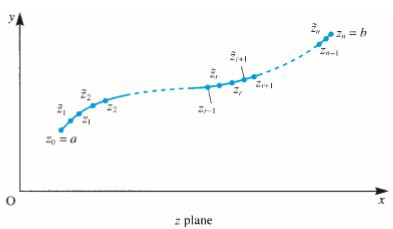
\includegraphics[]{Integral.JPG}
    \caption{Graphical representation of integration}
\end{figure}

By dividing the curve from $a$ to $b$ into $n$ parts with points $z_{n-1}$, the sum of the points
is:
$$
S_n = f(\hat{z}_1)(z_1-z_0)+f(\hat{z}_2)(z_2-z_1)+...+f(\hat{z}_n)(z_n-z_{n-1})
$$
The equation can be simplified into:
$$
S_n = \sum_{k=1}^n f(\hat{z}_k)\Delta z_k
$$

The \textbf{Contour Integral} is found when:
\begin{itemize}
    \item $n$ is the largest possible value such that difference between two points $|\Delta z_k|$ 
    approaches 0
    \item The sum $S_n$ approaches a limit (constant value)
\end{itemize}

\begin{tcolorbox}[breakable,colback=white]
\textbf{Contour Integral}:
$$
\int_C f(z)dz = \lim_{|\Delta z_k|\rightarrow 0} \sum_{k=1}^n f(\hat{z}_k) \Delta z_k
$$
where $z$ is defined as $z=x+\text{i }y$ thus $f(z)=u(x,y)+\text{i }v(x,y)$ \par 
$$
\int_C f(z)dz = \int_C [u(x,y)+\text{i }v(x,y)](dx+\text{i }dj)
$$
$$
\int_C f(z)dz = \int_C [u(x,y)dx - v(x,y)dy] + \text{i }\int_C [v(x,y)dx - u(x,y)dy]
$$
\end{tcolorbox}

\textbf{Example 1}: Evaluate contour integral $\int_C z^2$ along path $C$ listed below.
\begin{figure} [h!]
    \centering
    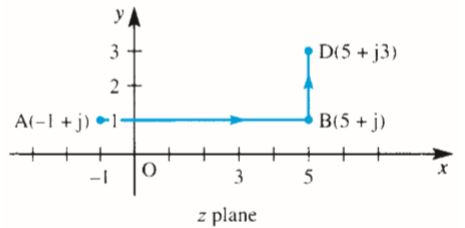
\includegraphics[scale=0.7]{Contour integral q.JPG}
    
\end{figure}

\begin{enumerate}
    \item Find $z^2$:
    \begin{equation*} 
        \begin{aligned}
            z^2 &= (x+jy)^2 \\
            &= (x^2 - y^2) + j2xy
        \end{aligned}
    \end{equation*}
    \item Define integral $I$:
    \begin{equation*} 
        \begin{aligned}
            z^2 &= \int_C z^2 dz \\
            &= \int_C [x^2 - y^2]\text{ dx} - 2xy \text{ dy}] + j\int_C [2xy\text{ dx}+(x^2 - y^2)\text{ dy}]
        \end{aligned}
    \end{equation*}
    \item The integral of AB ($y=1$ and $dy=0$):
    \begin{equation*} 
        \begin{aligned}
            I_{AB} &= \int_{-1}^5 (x^2 - 1)\text{ dx}+\text{j}\int_{-1}^5 2x \text{ dx} \\
            &= [\frac{1}{3}x^3 - x]_{-1}^5 + \text{j}[x^2]_{-1}^5 \\
            &= 36 + 24\text{j}
        \end{aligned}
    \end{equation*}
    \item The integral of BD ($x=5$ and $dx=0$):
    \begin{equation*} 
        \begin{aligned}
            I_{BD} &= \int_{1}^3 (-10y)\text{ dy}+\text{j}\int_{1}^3 (25-y^2) \text{ dy} \\
            &= [-5y^2]_1^3 + \text{j}[25y - \frac{1}{3}y^3]_1^3 \\
            &= 40+\text{j}\frac{124}{3}
        \end{aligned}
    \end{equation*}
    \item Combine the results:
    \begin{equation*} 
        \begin{aligned}
            \int_C z^2 \text{ dz} &= I_{AB} + I_{BD} \\
            &= (36 + \text{j}24) + (-40 + \text{j}\frac{124}{3}) \\
            &= -4 + \text{j}\frac{196}{3}
        \end{aligned}
    \end{equation*}
\end{enumerate}

%%%%%%%%%%%%%%%%%%%%%%%%%%%%%%%%%%%%%%%%%%%%%%%%%%%%%%%%%%%%%%%%%%%%%%%%%%%%%%%%%%%%%%%%%%%%%%%%%%%%%%%%%%
\subsection{Cauchy's theorem}

The most important theorem in complex variable theory and the foundation of complex variable
integration. \par 

\begin{tcolorbox}[breakable,colback=white]
If $f(z)$ has the following characteristics:
\begin{itemize}
    \item An analytic function with derivative $f'(z)$ 
    \item Continuous at all points inside 
    \item On a simple close curve $C$
\end{itemize}
\begin{center}
    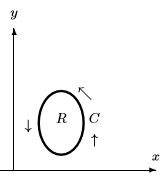
\includegraphics[scale=0.7]{Cauchy.JPG}
\end{center}
then: 
$$
\oint_C f(z) \text{ dz} = 0
$$
where $\oint_C$ denotes the integration \textbf{around a closed curve}.
\end{tcolorbox}

The proof of Cauchy's Theorem makes use of Green's Theorem in a plane. 

\begin{tcolorbox}[breakable,colback=white]
\textbf{Green's Theorem}: For differentiable functions $P(x,y)$ and $Q(x,y)$:
$$
\oint_C (P\text{ dx}+Q\text{ dy})=\int \int_R(Q_x - P_y) \text{dx dy}
$$ 
\end{tcolorbox}

\textbf{Proof}: \par 
Given the definition:
\begin{equation*} 
    \begin{aligned}
        \oint_C F(z)\text{ dz} &= \oint_C (u+iv)(dx +idy) \\
        &= \oint_C (u\text{ dx}-x\text{ dv})+ i\oint_C (v\text{ dx}+u\text{ dy})
    \end{aligned}
\end{equation*}

With the application of Green's Theorem:
\begin{equation*} 
    \begin{aligned}
        \oint (u\text{ dx}-v\text{ dy}) &= \int \int_R \int (-v_x-u_y)\text{dx dy} \\
        \oint (v\text{ dx}+u\text{ dy}) &= \int \int_R (u_x-v_y)\text{dx dy}
    \end{aligned}
\end{equation*}

These two combines into the final form: 
\begin{equation*} 
    \begin{aligned}
        \oint_C F(z)\text{ dz} = -\int \int_R (v_x+u_y)\text{dx dy} + i\int \int_R (u_x - v_y)\text{dx dy}
    \end{aligned}
\end{equation*}

If $F(z)$ is analytic everywhere on $C$ then $u$ and $v$ satisfies Cauchy-Riemann equations. This
means:
\begin{equation*} 
u_x = v_y \text{   and   } v_x=-u_y
\end{equation*}

This simplifies to Cauchy's Theorem: 
$$
\oint_C F(z) \text{ dz} = 0
$$

Cauchy's Theorem can be expressed alternatively with $z=a*e^{i\theta}$ for $\theta:0\rightarrow
2\pi$
\begin{equation*} 
    \begin{aligned}
        \oint_C \frac{dz}{z} &= \int_0^{2\pi}\frac{iae^{i\theta}\text{ d}\theta}{ae^{i\theta}} \\
        &= i \int_0^{2\pi}d\theta \\
        &= 2\pi i
    \end{aligned}
\end{equation*} 

\pagebreak

%%%%%%%%%%%%%%%%%%%%%%%%%%%%%%%%%%%%%%%%%%%%%%%%%%%%%%%%%%%%%%%%%%%%%%%%%%%%%%%%%%%%%%%%%%%%%%%%%%%%%%%%%%
\subsection{Residue Theorem}

The Residue Theorem is used to evaluate contour integrals and it draws from theories found in
differentiation and integration of complex functions.

\begin{tcolorbox}[breakable,colback=white]
\textbf{Residue Theorem}: If $f(z)$ is an analytic function within and on a simple closed curve $C$,
and the only singularities of $f(z)$ within $C$ are poles then:
$$
\oint_C f(z) \text{ dz} = 2\pi \text{i} \times \{\text{Sum of residues of $f(z)$ at its poles within $C$}\}
$$
\end{tcolorbox}

\textbf{Proof}:

\textbf{Example 1}: Find $\oint_{C_i} \frac{2z\text{ dz}}{(z-1)(z-2)}$ where:
\begin{itemize}
    \item $C_1$ is a circle centred at $(0,0)$ of radius 3
    \item $C_2$ is a circle centred at $(0,0)$ of radius $\frac{3}{2}$
\end{itemize}

Identifying the poles, $f(z)$ has two simple poles: $z=1$ and $z=2$ \par 

For $C_1$, both poles are inside $C_1$: 
\begin{equation*} 
    \begin{aligned}
        \oint_{C_1} f(z)\text{ dz} &= 2\pi \text{i} \times (-2 + 4) \\
        &= 4\pi \text{i}
    \end{aligned}
\end{equation*}

For $C_2$, only pole inside $C_2$ is $z=1$:
\begin{equation*} 
    \begin{aligned}
        \oint_{C_1} f(z)\text{ dz} &= 2\pi \text{i} \times (-2) \\
        &= -4\pi \text{i}
    \end{aligned}
\end{equation*}

\textbf{Example 2}: Find $\oint_{C} \frac{2z\text{ dz}}{(z-1)^2(z+4)}$ where $C$ circle has radius 5
centred at $z=0$. \par 

Identifying the poles, $f(z)$ has two simple poles: $z=1$ and $z=-4$ and both lie within $C$\par 
\begin{equation*} 
    \begin{aligned}
        \oint_{C} \frac{2z\text{ dz}}{(z-1)^2(z+4)} &= 2\pi \text{i} \times (-\frac{8}{25}+\frac{8}{25}) \\
        &= 0
    \end{aligned}
\end{equation*}

\textbf{Example 3}: Find $\oint_{C} \frac{z^2\text{ dz}}{(z-i)^3}$ where $C$ circle $|z|=2$
centred at $z=0$. \par 

Identifying the poles, $f(z)$ has a triple pole: $z=i$ \par
\begin{equation*} 
    \begin{aligned}
        \lim_{z\rightarrow 1}\frac{1}{2!}\frac{d^2}{dz^2}\left\{\frac{z^2(z-i)^3}{(z-1)^3}\right\}= 1\\
    \end{aligned}
\end{equation*}
Hence:
$$
\oint_{C} \frac{z^2\text{ dz}}{(z-i)^3} = 2\pi \text{i}
$$

%%%%%%%%%%%%%%%%%%%%%%%%%%%%%%%%%%%%%%%%%%%%%%%%%%%%%%%%%%%%%%%%%%%%%%%%%%%%%%%%%%%%%%%%%%%%%%%%%%%%%%%%%%
\subsection{Improper integrals and Jordan's Lemma}

The Residue Theorem is used to evaluate \textit{real integrals} of the following:
$$
\int_{-\infty}^{\infty} e^{imx}f(x)\text{ dx}
$$
where $m\geq 0$ \par 

\begin{tcolorbox}[breakable,colback=white]
\textbf{Improper Integrals}: A definite integral that has either or both limit of an infinite
nature.

\begin{equation*} 
    \begin{aligned}
        \int_{-\infty}^{\infty} e^{imx}f(x)\text{ dx} = \lim_{R\rightarrow \infty}\int_{-R}^R e^{imx}f(x) \text{ dx}
    \end{aligned}
\end{equation*}
\end{tcolorbox}

Jordan's lemma is a result frequently used in conjunction with the residue theorem to evaluate contour integrals and improper integrals. 

This is important as there is a class of Complex Integrals where $C$ consists of a semi-circle arc: \par
\begin{figure} [h!]
    \centering
    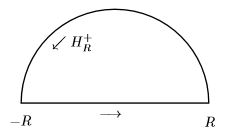
\includegraphics[]{Semicircle.JPG}
    
    \label{fig:Semicircle}
\end{figure}
where the semi-circle has radius $R$ and arc denoted $H_R$. The real axis has range $[-R,R]$. \par 

Building from the improper integral, it can be split into \textit{Real integral} and \textit{Complex
integral} and form the following equation for evaluation:

\begin{center}
    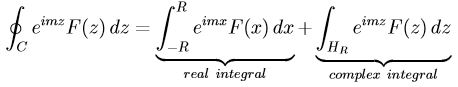
\includegraphics[scale=0.85]{Semi.JPG}
\end{center}

\begin{itemize}
    \item Complex integral: Evaluated with the Residue Theorem
    \item Real integral: Solving as $R\rightarrow \infty$ requires a result found in Jordan's Lemma.
\end{itemize}

%%%%%%%%%%%%%%%%%%%%%%%%%%%%%%%%%%%%%%%%%%%%%%%%%%%%%%%%%%%%%%%%%%%%%%%%%%%%%%%%%%%%%%%%%%%%%%%%%%%%%%%%%%
\subsubsection{Jordan's Lemma}

Jordan's Lemma deals with how a contour integral behaves on a semi-circular arc $H_R^+$ of a closed
contour $C$ such as Figure \ref{fig:Semicircle}

\begin{tcolorbox}[breakable,colback=white]
If the only singularities of $f(z)$ are poles then: 
$$
\lim_{R\rightarrow \infty} \int_{H_R} e^{imz}f(z) \text{ dz} = 0
$$
provided that $m>0$ and $|f(z)|\rightarrow 0$ as $R\rightarrow \infty$.
\\
\\
\textit{If $m=0$, a faster convergence to 0 is required for $f(z)$.}
\end{tcolorbox}

\textbf{Proof}: 
\\
\\
Since $H_R$ is a semi-circle:
\begin{equation*} 
    z=Re^{i\theta}=R(\cos(\theta)+\text{i}\sin(\theta))
\end{equation*}
\begin{center}
    and
\end{center}
\begin{equation*} 
    \text{dz} = \text{i}Re^{i\theta} \text{ d}\theta
\end{equation*}

Recall the following:
\begin{itemize}
    \item $|e^{i\alpha}|=1$ for any real $\alpha$
    \item $|\int f(z) \text{ dz}|\leq \int |f(z)| \text{ dz}$
\end{itemize}

Expand:
\begin{equation*} 
    \begin{aligned}
        \lim_{R\rightarrow \infty} \left|\int_{H_R}e^{imz}f(z)\text{ dz}\right|\ &= \lim_{R\rightarrow \infty} \left|\int_{H_R}e^{imR\cos \theta - mR\sin \theta}f(z)Re^{i\theta}\text{ d}\theta \right|\ \\
        &\leq \lim_{R\rightarrow \infty} \int_{H_R} e^{-mR\sin \theta} |f(z)|R \text{ d}\theta
    \end{aligned}
\end{equation*}

Provided $m>0$ as mentioned earlier, the exponential ensures that RHS is 0 in the limit
$R\rightarrow \infty$ thus satisfying the proof.

\textbf{Remarks}: 
\begin{enumerate}
    \item If $m>0$, forms of $f(z)$ will all converge fast enough due to all having simple poles and
    $|f(z)\rightarrow 0|$ as $R \rightarrow \infty$
    \item If $m=0$, alterations on the integer restrictions are required. E.g. $f(z)=\frac{1}{z}$
    then $|f(z)\rightarrow 0|$ but $\lim_R\rightarrow \infty |f(z)|=1$.
    \item If $m<0$, $\sin \theta < 0$ needs to ensure exponential is decreasing for $R\rightarrow \infty$.
    This is true in \textbf{lower half plane}, the contour taken in lower half plane $H_r^-$ but
    will still be in an anti-clockwise direction. 
\end{enumerate}

If $f(z)$ satisfies the conditions for Jordan's Lemma:
\small
$$
\int_{-\infty}^{\infty} e^{imx}f(x)\text{ dx} = 2\pi i \times \{\text{Sum of residues of poles of }e^{imzf(z)} \text{ in the upper }\frac{1}{2}\text{-plane} \}
$$


\textbf{Example 1}: Show that $\int_{-\infty}^{\infty} \frac{\text{dx}}{1+x^2} = \pi$ \par 

This problem can be solved simply with:
\begin{equation*} 
    \begin{aligned}
        I &= \lim_{R\rightarrow \infty}\int_{-R}^R \frac{\text{dx}}{1+x^2} \\
        &= \lim_{R\rightarrow \infty} [\tan^{-1}x]_{-R}^R \\
        &= \frac{\pi}{2}+\frac{\pi}{2} \\
        &= \pi
    \end{aligned}
\end{equation*}

Using Jordan's Lemma and Residue Theorem: 
\begin{figure} [h!]
    \centering
    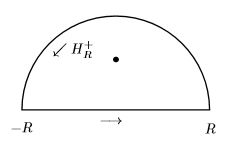
\includegraphics[scale=0.7]{Jordan_q.JPG}
    
\end{figure}

$C$ is comprised of a semi-circular arc $H_R^+$ and a section on real axis from $-R$ to $R$ with the
simple pole at $z=i$ lying within $C$. \par 

Considering the complex integral over $C$ in the upper half-plane with $m=0$: \par
$$
\oint_C \frac{\text{dz}}{1+z^2}
$$

The simple pole at $z=i$ and quadratic nature of denominator is enough for convergence thus Jordan's
Lemma:
$$
\lim_{R\rightarrow \infty} \int_{H_R} \frac{\text{dz}}{1+z^2} = 0
$$

Residue of $f(z)$ at the pole in upper-half plane at $z=i$ is $\frac{1}{2i}$ so Residue Theorem:
$$
\oint_C \frac{\text{dz}}{1+z^2} = 2\pi i \times \frac{1}{2i} = \pi
$$

\pagebreak

%%%%%%%%%%%%%%%%%%%%%%%%%%%%%%%%%%%%%%%%%%%%%%%%%%%%%%%%%%%%%%%%%%%%%%%%%%%%%%%%%%%%%%%%%%%%%%%%%%%%%%%%%%
\subsection{Integrals around the unit circle}

The integrals considered here are the type $\int_0^{2\pi}f(\cos \theta, \sin \theta) \text{
d}\theta$

\textbf{Working Example}: $I=\int_0^{2\pi} \frac{\text{d}\theta}{a+\cos \theta}$ where $a>1$ \par 

\begin{enumerate}
    \item Take $C$ as unit circle $z=e^{i\theta}$ thus $\text{dz}=ie^{i\theta}$
    \begin{equation*} 
        \begin{aligned}
            I &= \oint_C \frac{\text{dz}}{iz(a+\frac{1}{2}(z+z^{-1}))} \\
            &= -2i \oint_C \frac{\text{dz}}{z^2 + 2az + 1}
        \end{aligned}
    \end{equation*}
    \item Determine the roots of $z^2 + 2az + 1 = 0$
    $$
    z^2 + 2az + 1 = (z-\alpha^+)(z-\alpha^-)
    $$
    where $\alpha^{\pm} = -a \pm \sqrt{a^2 - 1}$ \par 
    When $a>1$ and:
    \begin{itemize}
        \item $\alpha^+$: Lies within $C$
        \item $\alpha^-$: Lies outside $C$
    \end{itemize}
    \item Compute the residue of the integrand at $z=\alpha^-$
    $$
    \frac{1}{\alpha^+ - \alpha^-}
    $$
    \item Use the Residue Theorem
    \begin{equation*} 
        \begin{aligned}
            T &= -2i \times 2\pi i \times \frac{1}{\alpha^+ - \alpha^-} \\
            &= \frac{2 \pi}{\sqrt{a^2 - 1}}
        \end{aligned}
    \end{equation*}
\end{enumerate}


%%%%%%%%%%%%%%%%%%%%%%%%%%%%%%%%%%%%%%%%%%%%%%%%%%%%%%%%%%%%%%%%%%%%%%%%%%%%%%%%%%%%%%%%%%%%%%%%%%%%%%%%%%
\subsection{Poles on Real axis}

If an integrand has a pole on the real axis, certain precautions need to be taken. \par 

\textbf{Working Example}: \par 

\begin{figure} [h!]
    \centering
    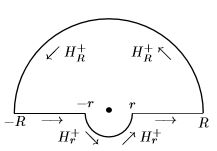
\includegraphics[]{Pole_real.JPG}
    
\end{figure}

Contour is deformed by small circle $H_r$ of radius $r$ at the origin excluding the pole at $z=0$. The big
semi-circle of radius $R$ is $H_R$.

Given: $\int_{-\infty}^{\infty}\frac{\sin x \text{ dx}}{x}$, we consider the complex integral
derived: $\oint_C \frac{e^{iz}\text{ dz}}{z}$ \par 

The integrand has no poles in $C$ since $z=0$ is excluded. Cauchy's Theorem is used:
\begin{equation*} 
    \begin{aligned}
        0 &= \oint_C \frac{e^{iz}\text{ dz}}{z} \\
        &= \int_{-R}^{-r} \frac{e^{ix}\text{ dx}}{x} + \int_{H_r \hookleftarrow} \frac{e^{iz} \text{ dz}}{z} + \int_r^R \frac{e^{ix}\text{ dx}}{x} + \int_{H_R \hookrightarrow} \frac{e^{iz}\text{ dz}}{z}
    \end{aligned}
\end{equation*}

Notice the following:
\begin{itemize}
    \item Take limit $R\rightarrow \infty$
    \item $m=1$ and Jordan's Lemma indicating that $\int_{H_R} = 0$ (Only singularity is a pole and
    integrand decays to 0 as $R\rightarrow \infty$)
    \item Small circle has equation $z=r(\cos \theta + i\sin \theta)$ and $\sin \theta \geq 0$
\end{itemize}
\begin{equation*} 
    \begin{aligned}
        \lim_{r\rightarrow 0}\int_{H_r} \frac{e^iz}{z} \text{ dz} &= i\lim_{r\rightarrow 0}\int_\pi^0 e^{-r\sin \theta}*e^{ir\cos \theta} \text{ d}\theta \\
        &= -\pi i
    \end{aligned}
\end{equation*}

Taking the two limit $R\rightarrow \infty$ and $r\rightarrow 0$:
$$
0 = \int_{-\infty}^\infty \frac{e^{ix}}{x} \text{ dx} - \pi i + 0
$$

Notice the real part of the integrand $\frac{\cos x}{x}$ is odd so contributions from $(-\infty,0)$
and $(0, \infty)$ cancel out: 
$$
\int_{\infty}^\infty \frac{\sin x}{x} \text{ dx} = \pi
$$


%%%%%%%%%%%%%%%%%%%%%%%%%%%%%%%%%%%%%%%%%%%%%%%%%%%%%%%%%%%%%%%%%%%%%%%%%%%%%%%%%%%%%%%%%%%%%%%%%%%%%%%%%%

\end{document}